\chapter{Detalles de Implementación}
\label{chapter:implementation}

\section{Introducción}

Este capítulo describe los principales aspectos relacionados con la implementación del sistema web desarrollado para el autorreporte y la gestión operativa de \gls{esavi}. 
El contenido aborda las tecnologías y herramientas incorporadas durante el desarrollo, la organización estructural de la solución y los mecanismos implementados tanto en el backend como en el frontend.

La implementación materializa las decisiones arquitectónicas definidas en el capítulo anterior mediante una arquitectura modular basada en los principios de Clean Architecture y Domain-Driven Design. 
La solución integra mecanismos de autenticación, comunicación asíncrona, persistencia de datos y validación de información, con el propósito de garantizar escalabilidad, mantenibilidad y seguridad.

Además, el capítulo expone los principales componentes funcionales de la plataforma, incluyendo el registro de reportes de ESAVI, la gestión de revisiones médicas, la asignación de responsables y el sistema de notificaciones. 
Finalmente, el contenido aborda elementos asociados al despliegue y la organización técnica de la aplicación.

\section{Tecnologías y herramientas utilizadas}
\label{section:technologies}

\subsection{Tecnologías del backend}

\textbf{C\# y .NET 8.} El backend se desarrolló en C\# sobre .NET 8, un framework de alto rendimiento que ofrece compilación nativa, inyección de dependencias integrada y un ecosistema maduro de bibliotecas para construir APIs REST. La documentación oficial de Microsoft establece que .NET 8 es la versión LTS (Long Term Support) recomendada para aplicaciones en producción \cite{dotnet8}.

\textbf{Entity Framework Core.} La persistencia de datos emplea Entity Framework Core como ORM (Object-Relational Mapper), que permite trabajar con la base de datos mediante objetos de C\# y expresiones LINQ sin escribir consultas SQL manualmente \cite{microsoft_efcore}.

\subsection{Tecnologías de la interfaz de usuario}

\textbf{React con TypeScript.} La interfaz de usuario se construye como una Single Page Application (SPA) en React, una biblioteca de JavaScript que permite crear interfaces interactivas mediante componentes reutilizables. TypeScript añade tipado estático sobre JavaScript, lo que reduce errores en tiempo de desarrollo y mejora la mantenibilidad del código.

\subsection{Sistema gestor de bases de datos}

\textbf{MySQL.} El sistema utiliza MySQL como motor de base de datos relacional. La documentación oficial de MySQL establece que su arquitectura de almacenamiento basada en tablas y su soporte para claves foráneas e índices lo hacen adecuado para aplicaciones que requieren integridad referencial estricta \cite{mysql_docs}. Esta característica resultó determinante para un dominio como el de farmacovigilancia, donde entidades como reportes, sujetos vacunados, revisores y vacunas deben mantener relaciones consistentes.

\subsection{Herramientas de infraestructura y despliegue}

\textbf{Docker.} La contenedorización de la aplicación empleó \textbf{Docker} para garantizar la consistencia entre los entornos de desarrollo, pruebas y producción. La documentación oficial de Docker establece que los contenedores empaquetan el código junto con todas sus dependencias, lo que asegura que el software funcione de manera uniforme en cualquier infraestructura \cite{docker-overview}. Esta característica elimina el clásico problema de ``en mi máquina funciona'' y facilita la distribución del proyecto.

\textbf{Railway.} El despliegue de la API, la base de datos MySQL y los servicios externos como RabbitMQ recayó en \textbf{Railway}, una plataforma como servicio que permite aprovisionar infraestructura en la nube y conectar el despliegue directamente con un repositorio de GitHub \cite{railway-docs}. Railway gestiona de forma automática las variables de entorno, los volúmenes de datos y la exposición de puertos, y activa una nueva construcción y publicación con cada cambio en la rama principal, lo que reduce significativamente el esfuerzo operativo durante el desarrollo \cite{railway-deployments}.

\textbf{Vercel.} Para el \textit{frontend}, el despliegue recayó en \textbf{Vercel}, una plataforma optimizada para aplicaciones web modernas que ofrece integración continua con repositorios de GitHub y distribución global mediante una red de entrega de contenido \cite{vercel-docs}.

Es importante señalar que tanto Railway como Vercel constituyen soluciones de desarrollo y demostración, adoptadas exclusivamente para facilitar que el equipo de investigadores del Instituto Finlay de Vacunas (IFV) y los tutores del proyecto pudieran observar los avances de forma remota y en tiempo real. La arquitectura del sistema está diseñada para migrar y contenerizar en servidores físicos dedicados del IFV cuando el proyecto transite a la etapa de producción, garantizando así el control institucional sobre los datos y la infraestructura.

\subsection{Herramientas de apoyo al desarrollo}

\textbf{Visual Studio Code.} El desarrollo del proyecto transcurrió en \textbf{Visual Studio Code}, con las extensiones oficiales para C\# y Docker. 
Microsoft recomienda este entorno para el desarrollo en .NET, ya que ofrece una integración completa con el SDK y la CLI de .NET \cite{vscode-dotnet}. 
Dicha integración permite crear, compilar y ejecutar aplicaciones directamente desde el editor, lo que agiliza el flujo de trabajo \cite{vscode-csharp}.

\textbf{Git y GitHub.} El control de versiones recayó con \textbf{Git} y el alojamiento del código en \textbf{GitHub}. 
GitHub proporciona un historial completo de cambios donde es posible consultar qué modificaciones ocurrieron, quién las hizo y por qué \cite{github-commits}. 
Al tratarse de un sistema distribuido, cada copia local del repositorio contiene el historial completo del proyecto, lo que permite recuperar cualquier estado anterior del código sin depender del servidor central \cite{pro-git-distributed}.

\textbf{Swagger (Swashbuckle).} Para documentar y probar la API, el proyecto incorporó \textbf{Swagger} a través de la librería Swashbuckle, que genera automáticamente una interfaz web con todos los endpoints, sus parámetros y permite ejecutar peticiones de prueba directamente desde el navegador \cite{swagger-ui}.



% \section{Estructura general de la solución}
% \label{section:solution_structure}

% \subsection{Organización de proyectos}

% \subsection{Separación por capas y responsabilidades}

% \subsection{Estructura modular del sistema}




\section{Implementación de la arquitectura}
\label{section:backend}

Una vez definida la arquitectura del sistema en la sección \ref{section:arquitectura}, este apartado describe cómo se materializaron las decisiones de diseño en código. 
La implementación sigue la estructura en capas propuesta por la arquitectura limpia: dominio, aplicación, infraestructura y presentación. Por cada capa se presentan los patrones utilizados, las tecnologías que los materializan y los fragmentos de código que ilustran las decisiones más relevantes.

\subsection{Capa de Dominio}

La capa de dominio constituye el núcleo del sistema y no depende de ningún otro proyecto de la solución ni de paquetes externos. 
Contiene las entidades de negocio, los objetos de valor, los enumerados, los eventos de dominio y las reglas intrínsecas del dominio de farmacovigilancia. 
Su independencia garantiza que los cambios en la infraestructura o en la presentación no afecten la lógica central del negocio.

\subsubsection{Entidades y agregados}

El diseño de las entidades parte del modelo de base de datos definido en el Capítulo 3. Cada tabla se modela como una clase de C\# que hereda de una jerarquía de clases base diseñada para unificar propiedades comunes y permitir la creación de interfaces genéricas en la capa de aplicación.

La jerarquía de herencia parte de \texttt{BasicEntity}, una clase abstracta que define las marcas de tiempo comunes a todas las entidades del sistema:

\begin{lstlisting}[language={[Sharp]C}, caption={Clase base BasicEntity con marcas de tiempo}, label={lst:basicentity}]
public abstract class BasicEntity
{
    public DateTime CreatedAt { get; set; }
    public DateTime UpdatedAt { get; set; }
}
\end{lstlisting}

Para contemplar entidades con distintos tipos de identificador, el dominio define la interfaz genérica \texttt{IEntity<TId>}:

\begin{lstlisting}[language={[Sharp]C}, caption={Interfaz genérica para identificadores de entidad}, label={lst:ientity}]
public interface IEntity<TId>
{
    TId Id { get; init; }
}
\end{lstlisting}

A partir de esta interfaz, el dominio proporciona dos clases abstractas especializadas. La clase \texttt{GuidEntity} constituye la norma para la mayoría de las entidades del sistema y utiliza un \texttt{Guid} como identificador:

\begin{lstlisting}[language={[Sharp]C}, caption={Clase GuidEntity para entidades con identificador Guid}, label={lst:guidentity}]
public abstract class GuidEntity : BasicEntity, IEntity<Guid>
{
    public Guid Id { get; init; } = new Guid();
}
\end{lstlisting}

Para entidades de catálogo que requieren un identificador entero —como las listas de provincias y municipios, cuyos registros son pocos, estables y no requieren las propiedades de seguridad de un \texttt{Guid}—, existe la clase \texttt{CatalogEntity}.

\begin{lstlisting}[language={[Sharp]C}, caption={Clase CatalogEntity para entidades con identificador entero}, label={lst:catalogentity}]
public abstract class CatalogEntity : BasicEntity, IEntity<int>
{
    public int Id { get; init; }
}
\end{lstlisting}

La elección de \texttt{Guid} como tipo de identificador para las entidades principales responde a criterios de seguridad y escalabilidad. La documentación oficial de Microsoft establece que un \texttt{Guid} (Globally Unique Identifier) es un número pseudoaleatorio de 128 bits con una probabilidad de colisión tan baja que resulta estadísticamente insignificante \cite{microsoft_guid}. A diferencia de los identificadores enteros autoincrementales, un \texttt{Guid} no revela la cantidad de registros en una tabla y no es predecible, lo que refuerza la seguridad de la aplicación. Esta propiedad permite, por ejemplo, exponer el identificador en una URL sin riesgo de que un usuario malintencionado itere sobre valores consecutivos.

Gracias a que \texttt{BasicEntity} unifica las propiedades comunes \texttt{CreatedAt} y \texttt{UpdatedAt}, la capa de aplicación puede definir interfaces genéricas que operan sobre cualquier entidad del sistema sin necesidad de implementaciones específicas por cada tipo. El siguiente fragmento, extraído de la capa de aplicación, ilustra esta ventaja:

\begin{lstlisting}[language={[Sharp]C}, caption={Interfaz genérica que opera sobre cualquier entidad que herede de BasicEntity}, label={lst:genericinterface}]
public interface IGenericRepository<T> where T : BasicEntity
{
    Task<T> GetByIdAsync<TId>(TId elementId);
    Task DeleteByIdAsync<TId>(TId elementId);
}
\end{lstlisting}

La restricción \texttt{where T : BasicEntity} garantiza en tiempo de compilación que la interfaz solo reciba entidades que posean las marcas de tiempo \texttt{CreatedAt} y \texttt{UpdatedAt}, independientemente del tipo de su identificador. Así, el sistema puede incorporar nuevas entidades —ya sea con \texttt{Guid} o con \texttt{int} como identificador— sin modificar las interfaces genéricas existentes, en cumplimiento del Principio de Abierto/Cerrado de \texttt{SOLID}.



\paragraph{Entidades User y Role}

Para la gestión de usuarios y roles, el proyecto emplea las clases \texttt{IdentityUser} y \texttt{IdentityRole} del paquete \texttt{Microsoft.AspNetCore.Identity}. Esta decisión evita implementar desde cero funcionalidades críticas como el almacenamiento seguro de contraseñas, la generación de tokens de verificación y el bloqueo de cuentas tras intentos fallidos.

La entidad \texttt{User} hereda de \texttt{IdentityUser<Guid>} y extiende el modelo con los campos requeridos por el dominio:

\begin{lstlisting}[language={[Sharp]C}, caption={Entidad User que hereda de IdentityUser<Guid>}, label={lst:user}]
public class User : IdentityUser<Guid>
{
    public Guid RoleId { get; set; }
    public DateTime CreatedAt { get; set; }
    public DateTime UpdatedAt { get; set; }
}
\end{lstlisting}

Aunque la clase derivada solo declara tres propiedades adicionales, la herencia de \texttt{IdentityUser<Guid>} aporta un conjunto completo de campos que cubren todas las necesidades de gestión de identidad \cite{microsoft_identity_model}. \texttt{UserName} almacena el nombre de usuario único para el inicio de sesión. \texttt{Email} contiene el correo electrónico empleado para notificaciones y verificación de cuenta. \texttt{PasswordHash} guarda el resultado del algoritmo de hashing y nunca contiene la contraseña en texto plano. \texttt{PhoneNumber} registra el teléfono para autenticación de dos factores o recuperación de cuenta. \texttt{EmailConfirmed} indica si el usuario verificó su correo electrónico. \texttt{LockoutEnd} establece la fecha y hora hasta la cual la cuenta permanece bloqueada tras superar el máximo de intentos fallidos. \texttt{AccessFailedCount} lleva el contador de intentos fallidos consecutivos. \texttt{SecurityStamp} almacena un valor aleatorio que cambia al modificar credenciales, lo que invalida automáticamente sesiones y tokens anteriores.

La entidad \texttt{Role} hereda de \texttt{IdentityRole<Guid>} y mantiene la misma coherencia en el tipo de identificador:

\begin{lstlisting}[language={[Sharp]C}, caption={Entidad Role que hereda de IdentityRole<Guid>}, label={lst:role}]
public class Role : IdentityRole<Guid>{ }
\end{lstlisting}

La herencia de \texttt{IdentityRole<Guid>} proporciona las propiedades \texttt{Name} (nombre único del rol) y \texttt{NormalizedName} (versión normalizada para búsquedas). 
La relación entre usuarios y roles sigue una restricción de uno a muchos: cada usuario posee un único rol mediante la clave foránea \texttt{RoleId} en la entidad \texttt{User}, mientras que un mismo rol puede agrupar a múltiples usuarios. 
Esta decisión simplifica la administración de permisos y refleja los perfiles definidos en el diseño del sistema (administrador, médico evaluador y jefe de vacunación municipal).


El uso de \texttt{Guid} como tipo de identificador en \texttt{IdentityUser} y \texttt{IdentityRole} mantiene la coherencia con la clase \texttt{GuidEntity} definida para el resto de las entidades del sistema, lo que permite que las tablas de identidad compartan el mismo tipo de clave primaria que las tablas de negocio.


\paragraph{Mecanismo de hashing de contraseñas}

La documentación oficial de Microsoft describe que el \texttt{PasswordHasher} de Identity implementa el algoritmo PBKDF2 (Password-Based Key Derivation Function 2), estándar del RFC 2898 que deriva una clave segura a partir de una contraseña \cite{rfc2898}. 
El algoritmo toma la contraseña del usuario, la combina con un \textit{salt} criptográficamente aleatorio de 128 bits y aplica repetidamente la función HMAC-SHA256\footnote{HMAC-SHA256: código de autenticación de mensajes basado en hash \cite{rfc2104}. Funciona aplicando de forma anidada el algoritmo SHA-256 a la combinación de una clave secreta (o \textit{salt}) con el mensaje. Internamente, la clave se procesa mediante una operación XOR con una secuencia de relleno interna (\textit{ipad}) antes de aplicar el primer hash al mensaje; posteriormente, el resultado se combina mediante XOR con una secuencia externa (\textit{opad}) y se somete a un segundo hash SHA-256, garantizando simultáneamente la integridad y autenticidad del resultado.}
durante 100,000 iteraciones como valor predeterminado \cite{microsoft_password_hasher}. Cada iteración adicional duplica el costo computacional de un ataque por fuerza bruta sin afectar perceptiblemente el tiempo de verificación para un usuario legítimo. El formato del hash generado produce una cadena con la siguiente estructura \cite{microsoft_hash_format}:

\begin{center}
\texttt{Base64(salt).Base64(subkey)}
\end{center}

Donde el \textit{salt} es un valor aleatorio único por cada contraseña y el \textit{subkey} es el resultado de aplicar PBKDF2 durante el número configurado de iteraciones.

Este mecanismo garantiza tres propiedades de seguridad esenciales:

\begin{itemize}
    \item \textbf{Unicidad del hash:} dos usuarios con la misma contraseña producen hashes completamente diferentes porque el \textit{salt} generado para cada uno es distinto. Esto impide que un atacante compare hashes para identificar contraseñas idénticas dentro de una base de datos comprometida \cite{owasp_password_storage}.
    
    \item \textbf{Irreversibilidad computacional:} PBKDF2 es una función unidireccional. El elevado número de iteraciones convierte el cálculo del hash en un proceso deliberadamente costoso en tiempo de CPU, lo que ralentiza significativamente cualquier intento de ataque por fuerza bruta incluso si el atacante posee hardware especializado \cite{microsoft_password_hasher}.
    
    \item \textbf{Invalidación de sesiones previas:} la propiedad \texttt{SecurityStamp}, generada aleatoriamente y modificada cada vez que el usuario cambia su contraseña, se incluye en la generación de tokens de autenticación. Si un atacante obtiene credenciales antiguas, el cambio de \texttt{SecurityStamp} invalida inmediatamente cualquier sesión o token previo \cite{microsoft_security_stamp}.
\end{itemize}

La verificación de la contraseña durante el inicio de sesión se realiza internamente mediante el método \texttt{VerifyHashedPassword}, que recalcula el hash con el \textit{salt} almacenado y compara los resultados en tiempo constante, sin que la aplicación necesite conocer el texto plano de la contraseña en ningún momento \cite{microsoft_password_hasher}.





\paragraph{Generación de tokens para verificación de identidad}

El paquete Identity incluye proveedores de tokens integrados que generan cadenas criptográficamente seguras para distintos propósitos. 
El sistema emplea estos tokens durante el proceso de registro para verificar que un usuario controla la dirección de correo electrónico declarada y para permitir el establecimiento seguro de su contraseña inicial. 
La documentación oficial explica que el proveedor predeterminado \texttt{DataProtectorTokenProvider} utiliza internamente la API de Protección de Datos de ASP.NET Core, la cual aplica cifrado autenticado (AES-256-CBC\footnote{AES-256-CBC (Advanced Encryption Standard con modo Cipher Block Chaining y clave de 256 bits): algoritmo de cifrado simétrico estandarizado por el Instituto Nacional de Estándares y Tecnología (NIST, por sus siglas en inglés), agencia del gobierno de Estados Unidos. Transforma datos legibles en texto cifrado usando una clave secreta, y el modo CBC garantiza que mensajes idénticos produzcan resultados cifrados diferentes \cite{nist_aes}.} con HMAC-SHA256) sobre los datos del token \cite{microsoft_token_providers}. 
Esto garantiza tres propiedades de seguridad esenciales: el token no revela información del usuario si es interceptado, cualquier modificación invalida la firma y provoca el rechazo del servidor, y un atacante no puede generar un token válido sin acceder a las claves de protección del servidor \cite{microsoft_data_protection}.

El token posee una vigencia predeterminada de 24 horas, controlada por la propiedad \texttt{TokenLifespan} de \texttt{DataProtectionTokenProviderOptions}, transcurrida la cual expira automáticamente \cite{microsoft_identity_config}. 
La validación ocurre en el servidor sin necesidad de consultar una tabla de tokens pendientes, lo que simplifica la arquitectura y elimina la necesidad de limpiar tokens expirados. 
El caso de uso concreto que orquesta la generación y validación de estos tokens durante el registro de médicos evaluadores se detalla en la sección dedicada a la capa de aplicación.

\paragraph{Configuración de seguridad adicional}

Además de los valores predeterminados, el proyecto configura el número de iteraciones del algoritmo PBKDF2 a 600,000 mediante la clase \texttt{PasswordHasherOptions}:

\begin{lstlisting}[language={[Sharp]C}, caption={Configuración de iteraciones de hashing en Program.cs}, label={lst:passwordoptions}]
builder.Services.Configure<PasswordHasherOptions>(options =>
{
    options.IterationCount = 600_000;
});
\end{lstlisting}

Este ajuste sigue las recomendaciones actuales de OWASP para el algoritmo PBKDF2-SHA256, que establecen un mínimo de 600,000 iteraciones para aplicaciones desplegadas en entornos de producción \cite{owasp_password_storage}. El incremento respecto al valor predeterminado de 100,000 iteraciones aumenta el costo computacional de cada intento de verificación de contraseña en un factor de seis, lo que dificulta aún más los ataques de diccionario sin afectar perceptiblemente el tiempo de inicio de sesión de un usuario legítimo.



\subsubsection{Objetos de valor}

El dominio incluye el objeto de valor \texttt{IdentityNumber}, que encapsula la validación del formato del carné de identidad cubano, la extracción de la fecha de nacimiento y el cálculo de la edad. Esta decisión responde a que varias entidades del sistema —\texttt{VaccinatedSubject}, \texttt{Reporter} y \texttt{MedicalReviewer}— contienen un carné de identidad y requieren las mismas operaciones sobre él. Al extraer esta lógica en un objeto de valor inmutable, se evita la duplicación de código y se garantiza que cualquier validación o cálculo sobre el carné se aplique de manera uniforme en todo el sistema.

\subsubsection{Enumerados}

Los enumerados representan clasificaciones propias del negocio cuyos valores no cambian durante la ejecución de la aplicación. El dominio los define mediante el tipo \texttt{enum} de C\#, lo que garantiza que toda la aplicación comparta las mismas categorías sin riesgo de discrepancias entre capas. Estos tipos no constituyen entidades ni tablas en la base de datos porque sus valores son fijos y no requieren persistencia independiente.

En contraste, conceptos como \texttt{Province} y \texttt{Municipality} sí se modelan como entidades y tablas. Existe una relación entre ambos —cada municipio pertenece a una provincia— que resulta más clara de expresar mediante llaves foráneas que mediante un enumerado extenso. Además, el sistema realiza operaciones frecuentes de búsqueda y filtrado sobre estos datos, para las cuales una tabla indexada ofrece mejor rendimiento. Por último, la lista de provincias y municipios puede actualizarse ocasionalmente por cambios administrativos, y una tabla permite modificarla sin recompilar la aplicación.


\subsubsection{Eventos de dominio}

Los eventos de dominio representan sucesos relevantes del negocio que otras partes del sistema deben conocer. El proyecto los define como clases simples con propiedades que identifican los datos del suceso y los utiliza para desencadenar el envío de notificaciones por correo electrónico sin acoplar la lógica de envío a las entidades. Esta arquitectura mantiene el dominio aislado de los detalles de infraestructura y permite agregar nuevos manejadores sin modificar las entidades ni los casos de uso.

Durante la implementación surgieron además dos entidades de infraestructura no previstas en el diseño inicial: \texttt{RefreshToken}, que permite la renovación de sesiones sin reautenticación, y \texttt{AuditLog}, que registra las operaciones realizadas sobre el sistema con fines de trazabilidad. Ambas heredan de \texttt{GuidEntity} y su definición detallada se presenta en el Anexo \ref{anexo:entidades_infraestructura}.



\subsection{Capa de Aplicación}
\label{subsection:aplicacion}

La capa de aplicación orquesta los casos de uso del sistema. Recibe comandos y consultas desde la capa de presentación, coordina las entidades del dominio y los servicios de infraestructura, y retorna resultados transformados en DTOs. Esta capa depende exclusivamente del dominio, por lo que desconoce los detalles de la base de datos, el envío de correos o la generación de tokens.

\subsubsection{Casos de uso y servicios de aplicación}

Los casos de uso se implementan mediante servicios de aplicación que el controlador invoca a través de interfaces. Esta decisión responde al patrón de Inyección de Dependencias (Dependency Injection, DI): en lugar de que cada clase cree sus propias dependencias mediante \texttt{new}, el contenedor de DI de ASP.NET Core las suministra automáticamente al constructor. 
El desarrollador registra qué implementación concreta corresponde a cada interfaz, y el contenedor resuelve las dependencias en tiempo de ejecución \cite{ms_di_doc}.

Este patrón resuelve un problema concreto de acoplamiento. Sin DI, la capa de presentación necesitaría conocer las clases concretas de la capa de aplicación para instanciarlas. Con DI, la presentación solo declara la interfaz en su constructor, sin saber qué implementación recibe ni dónde se encuentra. 
Así, si la lógica de negocio cambia, solo debe modificarse la capa de aplicación; la presentación permanece intacta. Este mismo principio se aplica en todas las capas del sistema: la capa de aplicación declara interfaces de repositorio que la infraestructura implementa, y la capa de infraestructura declara interfaces de servicios externos que los proveedores concretos satisfacen. 
El contenedor centraliza las dependencias en métodos como \texttt{AddAplication} e \texttt{AddInfrastructure}:

\begin{lstlisting}[language={[Sharp]C}, caption={Registro de servicios en el contenedor de DI}, label={lst:di_registration}]
// Capa de aplicación: AddAplication
services.AddScoped<IReportCommandService, ReportCommandService>();
services.AddScoped<IReportQueryService, ReportQueryService>();
services.AddScoped<IIdentityService, IdentityService>();

// Capa de infraestructura: AddInfrastructure
services.AddScoped<IUnitOfWork, UnitOfWork>();
services.AddScoped<IJwtTokenGenerator, JwtTokenGenerator>();
services.AddScoped<IEmailService, EmailJsService>();
\end{lstlisting}

El siguiente fragmento muestra cómo el controlador recibe \texttt{IIdentityService} sin conocer su implementación, y cómo el servicio de aplicación recibe a su vez \texttt{IJwtTokenGenerator} y \texttt{IUnitOfWork} bajo el mismo principio:

\begin{lstlisting}[language={[Sharp]C}, caption={Inyección de abstracciones en todas las capas}, label={lst:di_controller}]
// Capa de presentación: solo conoce la interfaz
public class AuthenticationController : ControllerBase
{
    private readonly IIdentityService _identityService;

    public AuthenticationController(IIdentityService identityService)
    {
        _identityService = identityService;
    }
}

// Capa de aplicación: recibe interfaces, no implementaciones
public class IdentityService : IIdentityService
{
    private readonly IJwtTokenGenerator _jwtTokenGenerator;
    private readonly IUnitOfWork _unitOfWork;

    public IdentityService(
        IJwtTokenGenerator jwtTokenGenerator,
        IUnitOfWork unitOfWork)
    {
        _jwtTokenGenerator = jwtTokenGenerator;
        _unitOfWork = unitOfWork;
    }
}
\end{lstlisting}

El sistema aplica además el Principio de Separación de Comandos y Consultas (CQS), propuesto por Bertrand Meyer, que establece que una operación debe ser un comando —modifica el estado sin retornar datos— o una consulta —retorna datos sin modificar el estado—, pero nunca ambas cosas \cite{Meyer1988}. 
Llevado a la arquitectura, cada recurso del dominio define dos interfaces: una para comandos y otra para consultas. 
El siguiente fragmento muestra esta separación para el recurso de reportes:

\begin{lstlisting}[language={[Sharp]C}, caption={Separación CQS en interfaces de reportes}, label={lst:cqs}]
// Comandos: modifican el estado
public interface IReportCommandService
{
    Task<Guid> CreatePublicReportAsync(PublicAefiReportDto dto);
    Task CompleteReviewAsync(CompleteReviewDto dto);
}

// Consultas: retornan datos sin modificar
public interface IReportQueryService
{
    Task<PagedResultDto<ReportDto>> GetReportsAsync(PagedRequestDto paged);
    Task<ReportDto> GetReportByNotificationNumber(string notificationNumber);
}
\end{lstlisting}

Esta separación no alcanza la complejidad de un CQRS completo —ambos servicios comparten el mismo modelo de dominio y la misma base de datos—, pero permite que cada interfaz evolucione según sus necesidades específicas.

Los servicios de aplicación coordinan los repositorios y el Unit of Work para ejecutar los casos de uso. El siguiente fragmento, extraído de \texttt{IdentityService}, muestra cómo un caso de uso orquesta múltiples dependencias dentro de una misma transacción:

\begin{lstlisting}[language={[Sharp]C}, caption={Orquestación de dependencias en un caso de uso}, label={lst:orchestration}]
public async Task<UserResponseDTO> LoginUserAsync(LoginUserDto loginDto)
{
    var savedUser = await _identityManager.CheckCredentialsAsync(
        loginDto.Email, loginDto.Password)
        ?? throw new ArgumentException("Invalid credentials");

    var accessToken = await _jwtTokenGenerator.GenerateToken(savedUser);
    var refreshToken = GenerateRefreshToken();

    await _unitOfWork.GetRepository<RefreshToken>().CreateAsync(
        new RefreshToken
        {
            Token = refreshToken,
            ExpiresAt = DateTime.UtcNow.AddDays(7),
            UserId = savedUser.Id
        });

    await _unitOfWork.CompleteAsync();

    return new UserResponseDTO { ... };
}
\end{lstlisting}

\subsubsection{Mapeo y transformación de datos}

La capa de aplicación define DTOs (Data Transfer Objects, objetos de transferencia de datos) para mover información entre la API y el dominio. Un DTO es un objeto plano que contiene solo propiedades, sin lógica de negocio, diseñado para transportar datos en un formato adecuado para el cliente. Las entidades del dominio no se exponen fuera de esta capa, lo que protege al núcleo del sistema de cambios en los formatos de intercambio y evita la exposición accidental de propiedades internas.

El sistema emplea AutoMapper para convertir entidades en DTOs y viceversa, aplicando el patrón Mapper \cite{fowler_mapper}. 
AutoMapper permite definir reglas de transformación en clases llamadas perfiles, que heredan de \texttt{Profile} y centralizan las conversiones entre tipos. 
Cada perfil declara cómo se asigna cada propiedad de un tipo origen a un tipo destino, incluyendo propiedades anidadas que requieren lógica adicional:

\begin{lstlisting}[language={[Sharp]C}, caption={Perfil de mapeo con AutoMapper}, label={lst:mapper_profile}]
public class AefiReportProfile : Profile
{
    public AefiReportProfile()
    {
        CreateMap<AefiReport, ReportDto>()
            .ForMember(dest => dest.SubjectName,
                opt => opt.MapFrom(src => src.VaccinatedSubject.FullName))
            .ForMember(dest => dest.VaccineNames,
                opt => opt.MapFrom(src => src.Vaccinations
                    .Select(v => v.Lot.Vaccine.Name)));
    }
}
\end{lstlisting}

En este ejemplo, \texttt{SubjectName} no existe directamente en \texttt{AefiReport}, sino que se obtiene navegando la relación hacia \texttt{VaccinatedSubject}. 
AutoMapper resuelve esta navegación automáticamente y genera la consulta SQL correspondiente.

Para las consultas, el sistema aprovecha el método \texttt{ProjectTo<T>} de AutoMapper. 
A diferencia de un mapeo en memoria —que cargaría la entidad completa para luego transformarla—, \texttt{ProjectTo} traduce la proyección directamente a SQL, de modo que solo las columnas necesarias viajan desde la base de datos hasta la aplicación:

\begin{lstlisting}[language={[Sharp]C}, caption={Proyección directa a DTO con ProjectTo}, label={lst:projectto}]
var items = await _unitOfWork.GetRepository<AefiReport>()
    .GetPaged(query, skip, take)
    .ProjectTo<ReportDto>(_mapper.ConfigurationProvider)
    .ToListAsync();
\end{lstlisting}

Esta técnica mejora el rendimiento de las consultas al evitar la carga completa de las entidades y sus relaciones, y al delegar la selección de columnas al motor de base de datos.


\subsubsection{Validaciones y manejo de solicitudes}

El sistema aplica dos niveles de validación sobre cada solicitud entrante, en momentos distintos del procesamiento y con propósitos complementarios.

El primer nivel opera sobre los DTOs mediante atributos de validación de .NET. 
Estos atributos verifican condiciones simples —obligatoriedad, longitud máxima, formato de correo electrónico o número de teléfono— antes de que la solicitud alcance el servicio de aplicación. ASP.NET Core ejecuta esta validación automáticamente al construir el DTO desde el cuerpo de la solicitud, gracias al atributo \texttt{[ApiController]}. 
Si algún atributo falla, el middleware devuelve un código 400 con los campos que incumplieron la validación. El siguiente fragmento muestra un DTO con atributos de validación estándar y personalizados:

\begin{lstlisting}[language={[Sharp]C}, caption={DTO con atributos de validación}, label={lst:dto_validation}]
public class VaccinatedSubjectDto
{
    [Required(ErrorMessage = "Full name is required.")]
    [StringLength(150, MinimumLength = 1)]
    public string FullName { get; set; } = string.Empty;

    [Required(ErrorMessage = "Identity number is required.")]
    [IdentityNumberValidation]
    public string IdentityNumber { get; set; } = string.Empty;
    
    // el resto de atributos
}
\end{lstlisting}

Los atributos personalizados \texttt{IdentityNumberValidation} y \texttt{EmailValidation}, definidos en la capa de aplicación, heredan de \texttt{ValidationAttribute} y encapsulan reglas reutilizables sin duplicar código en múltiples DTOs:

\begin{lstlisting}[language={[Sharp]C}, caption={Atributo de validación personalizado}, label={lst:custom_validation}]
public class IdentityNumberValidationAttribute : ValidationAttribute
{
    protected override ValidationResult? IsValid(object? value,
        ValidationContext validationContext)
    {
        // valida que tenga formato de 11 dígitos y coherencia
        return ValidationResult.Success;
    }
}
\end{lstlisting}

El segundo nivel opera dentro del servicio de aplicación, una vez que la solicitud superó las validaciones de formato. Este nivel aplica reglas de negocio que requieren consultar la base de datos o comparar datos de múltiples fuentes: verificar que una vacuna exista, que un lote pertenezca a la vacuna declarada, o que la fecha de administración de la vacuna no sea posterior a la fecha de inicio de los síntomas. Para ello, el sistema define la interfaz \texttt{IReportValidator<T>} y la inyecta en los servicios de aplicación mediante el contenedor de dependencias:

\begin{lstlisting}[language={[Sharp]C}, caption={Inyección de validadores en el servicio de aplicación}, label={lst:validator_injection}]
public class ReportCommandService : IReportCommandService
{
   // constructor de la clase y variables privadas
   
    public async Task<CreateReportResponseDto> CreatePublicReportAsync(
        PublicAefiReportDto reportDto)
    {
        // Ejecuta todos los validadores registrados para este tipo de DTO
        foreach (var validator in _validators)
            await validator.ValidateAsync(reportDto);

        // Continúa con la creación del reporte...
    }
}
\end{lstlisting}

El contenedor de dependencias resuelve automáticamente todas las implementaciones de \texttt{IReportValidator<T>} registradas y las inyecta como una colección. Esto permite que el servicio ejecute todos los validadores sin conocer sus tipos concretos, en cumplimiento del Principio de Abierto/Cerrado: agregar una nueva regla de validación solo requiere implementar la interfaz y registrarla en el contenedor, sin modificar el servicio de aplicación.

Este mismo patrón de validación en segundo nivel aplica a otras reglas de negocio que operan sobre datos ya persistidos. 
Un ejemplo es la expiración de asignaciones, implementada en \texttt{IAssignmentExpirationService}. 
Esta regla materializa RN-07 y RN-08 (Capítulo \ref{chapter:proposal}): determina la prioridad del reporte a partir del evento adverso más grave que contenga y aplica el plazo de evaluación correspondiente —24 horas para prioridad alta, 5 días para prioridad media y 7 días para prioridad baja—. 
El servicio consulta las asignaciones pendientes, compara su fecha de asignación con el plazo según la prioridad del reporte asociado y marca como expiradas aquellas que lo superan.

La capa de aplicación extiende el principio de inversión de dependencias a los servicios de infraestructura que necesita para completar sus casos de uso.
Para acceder a los datos, la aplicación declara interfaces de repositorio como \texttt{IGenericRepository<T>} y \texttt{IUserRepository}, cuyas implementaciones residen en la capa de infraestructura. Para enviar notificaciones, declara \texttt{IEmailService} sin saber si el envío utiliza un servicio externo, un servidor SMTP o cualquier otro mecanismo. Para la autenticación, declara \texttt{IJwtTokenGenerator} e \texttt{IIdentityManager} sin conocer los algoritmos de firma ni las claves secretas. 
En cada caso, el servicio de aplicación solo conoce la interfaz y confía en que el contenedor de DI suministrará la implementación registrada en \texttt{AddInfrastructure}. Esta separación permite cambiar el proveedor de correo electrónico, el motor de base de datos o el servicio de CAPTCHA sin modificar una sola línea de la capa de aplicación.







\subsection{Capa de Infraestructura}

La capa de infraestructura implementa los contratos definidos en las capas de dominio y aplicación. Contiene el acceso a la base de datos, la generación de tokens, el envío de correos electrónicos, la mensajería asíncrona y la integración con servicios externos. Todas las dependencias hacia el mundo exterior residen aquí, lo que permite que el núcleo del sistema permanezca independiente de tecnologías concretas.


\subsubsection{Persistencia de datos y configuración de Entity Framework Core}

El sistema utiliza MySQL como motor de base de datos relacional. 
La conexión se establece mediante una cadena de conexión —que contiene el servidor, el nombre de la base de datos y las credenciales de acceso— almacenada en las variables de entorno del servidor bajo el nombre \texttt{AppDbConnectionString}. 
El paquete Pomelo.EntityFrameworkCore.MySql, un proveedor de .NET que adapta Entity Framework Core a las características específicas de MySQL \cite{mysql_efcore}, toma esta cadena y la utiliza para establecer la comunicación con la base de datos. 
La configuración se realiza durante el arranque de la aplicación, en un método de extensión llamado \texttt{AddInfrastructure} que centraliza el registro de todos los servicios de esta capa en el contenedor de inyección de dependencias:

\begin{lstlisting}[language={[Sharp]C}, caption={Configuración de la conexión a MySQL}, label={lst:mysqlconfig}]
var connectionString = configuration.GetConnectionString("AppDbConnectionString");
services.AddDbContext<FinlayDbContext>(options =>
    options.UseMySql(connectionString, ServerVersion.AutoDetect(connectionString)));
\end{lstlisting}

Sobre esta conexión, el contexto \texttt{FinlayDbContext} —la clase que representa la sesión con la base de datos— centraliza el acceso a todas las tablas del sistema. 
Las características de infraestructura de cada tabla se definen en el método \texttt{OnModelCreating} mediante la API fluida de Entity Framework Core, sin decorar las clases del dominio con atributos propios de la persistencia \cite{microsoft_efcore}. 
Este método aplica las mismas restricciones definidas en el diseño de la base de datos (Capítulo 3, Sección 3.5): nulabilidad, longitudes máximas, llaves foráneas e índices\footnote{Un índice es una estructura de datos que permite al motor de base de datos localizar filas sin recorrer toda la tabla, de forma similar al índice alfabético de un libro. El sistema define índices sobre columnas consultadas con frecuencia.}.
Además, cada relación declara un comportamiento de borrado y actualización: \texttt{Cascade} propaga la operación cuando la entidad dependiente carece de sentido sin su principal, mientras que \texttt{Restrict} la bloquea si existen registros referenciados desde otra tabla. 
El siguiente fragmento, correspondiente a la entidad \texttt{AefiReport}, ilustra estas decisiones:

\begin{lstlisting}[language={[Sharp]C}, caption={Configuración de infraestructura para AefiReport}, label={lst:fluentapi}]
builder.Entity<AefiReport>(entity =>
{
    entity.HasKey(e => e.Id);
    entity.Property(e => e.NotificationNumber)
          .IsRequired()
          .HasMaxLength(100);
    entity.HasIndex(e => e.NotificationNumber).IsUnique();
    entity.HasOne(r => r.VaccinatedSubject)
          .WithMany(p => p.AefiReports)
          .HasForeignKey(r => r.VaccinatedSubjectId)
          .OnDelete(DeleteBehavior.Restrict);

    // otros atributos y llaves foráneas
});
\end{lstlisting}


\subsubsection{Migraciones y acceso a datos}

El acceso a los datos se implementa mediante el patrón Repository, que abstrae las operaciones de persistencia detrás de interfaces definidas en la capa de aplicación. La clase \texttt{GenericRepository<T>} proporciona una implementación genérica para operaciones comunes —crear, obtener por identificador, listar, actualizar y eliminar— y aprovecha la restricción \texttt{where T : BasicEntity} para operar sobre cualquier entidad del sistema sin duplicar código:

\begin{lstlisting}[language={[Sharp]C}, caption={Repositorio genérico}, label={lst:genericrepository}]
public class GenericRepository<T> : IGenericRepository<T> where T : BasicEntity
{
    protected readonly DbSet<T> _entity;

    public virtual async Task<T> CreateAsync(T element) { ... }
    public virtual async Task<T> GetByIdAsync<TId>(TId elementId) { ... }
    public virtual IQueryable<T> GetAll() { ... }
    public virtual void Update(T element) { ... }
    public virtual async Task DeleteByIdAsync<TId>(TId elementId) { ... }
}
\end{lstlisting}

Cuando una entidad requiere consultas que el repositorio genérico no cubre, el sistema define repositorios especializados que heredan de \texttt{GenericRepository<T>} y añaden métodos particulares. Todas las consultas utilizan LINQ, el lenguaje de consulta integrado de C\#, que Entity Framework Core traduce automáticamente a SQL. El siguiente ejemplo muestra una consulta LINQ y la sentencia SQL equivalente que se ejecuta en la base de datos:

\begin{lstlisting}[language={[Sharp]C}, caption={Consulta LINQ y su traducción a SQL}, label={lst:linq}]
// LINQ
var reportes = await _entity
    .Where(r => r.Status == AefiReportStatus.UnderReview)
    .OrderByDescending(r => r.ReportDate)
    .Take(10)
    .ToListAsync();

// SQL generado
SELECT TOP 10 *
FROM AefiReports
WHERE Status = 'UnderReview'
ORDER BY ReportDate DESC;
\end{lstlisting}

El patrón Unit of Work, implementado en la clase \texttt{UnitOfWork}, coordina las operaciones de múltiples repositorios dentro de una única transacción. 
Su método \texttt{CompleteAsync} invoca \texttt{SaveChangesAsync} del contexto. 
Esto garantiza que todos los cambios realizados durante un caso de uso se persistan de forma atómica: si cualquier operación falla, ninguna se materializa en la base de datos \cite{martin_fowler_uow}.

El registro de auditoría se implementa mediante un interceptor de Entity Framework Core que hereda de \texttt{SaveChangesInterceptor}. 
Este interceptor se ejecuta automáticamente antes de cada \texttt{SaveChangesAsync}: recorre las entidades modificadas, serializa los valores anteriores y posteriores de cada operación, y añade los registros correspondientes a la tabla \texttt{AuditLog}. 
Como el interceptor opera dentro de la misma transacción, la auditoría y los cambios de negocio se persisten de forma atómica. 
Esta solución mantiene la transparencia para los casos de uso, que no necesitan invocar ningún servicio de auditoría.

\subsubsection{Integración con servicios externos}

El sistema integra cuatro servicios externos principales: 


\textbf{Friendly CAPTCHA\footnote{CAPTCHA (Completely Automated Public Turing test to tell Computers and Humans Apart): prueba de Turing automatizada que distingue a un humano de un ordenador.}.} Los endpoints públicos están expuestos a ataques automatizados que envían solicitudes directamente a la API. Como primera barrera, el sistema utiliza Friendly CAPTCHA, un servicio de verificación basado en prueba de trabajo criptográfica (proof-of-work) que no afecta la experiencia del usuario. La sección de seguridad (Apartado \ref{section:seguridad}) detalla el fundamento y el flujo de verificación de este mecanismo.

\textbf{Notificaciones por correo electrónico y WhatsApp.} El sistema necesita notificar a los usuarios sobre eventos relevantes —confirmación de reporte, asignación a revisor, expiración de asignación— a través de canales accesibles para la población cubana. La vía de SMS resultó inviable para esta etapa por razones de infraestructura y costo, por lo que el sistema adopta el correo electrónico y WhatsApp, las dos vías con mayor penetración en la ciudadanía cubana.

\textbf{EmailJS.} Para el envío de correos electrónicos, el sistema utiliza EmailJS, un servicio que permite enviar correos sin configurar un servidor SMTP propio. 
El servicio \texttt{EmailJsService} implementa la interfaz \texttt{IEmailService} y construye una solicitud HTTP a la API de EmailJS con los parámetros de la plantilla, el identificador del servicio y el token de acceso, todos configurados en \texttt{EmailJsSettings}:

\begin{lstlisting}[language={[Sharp]C}, caption={Envío de correo mediante EmailJS}, label={lst:emailjs}]
var payload = new
{
    service_id = _settings.ServiceId,       
    template_id = templateId,                
    user_id = _settings.UserId,             
    accessToken = _settings.AccessToken,   
    template_params = templateParams          // diccionario que tiene los datos específicos de la plantilla
};

// Serializar y enviar la solicitud a la API de EmailJS
var json = JsonSerializer.Serialize(payload);
var content = new StringContent(json, Encoding.UTF8, "application/json");
var response = await _httpClient.PostAsync(url, content);
\end{lstlisting}

Cada tipo de notificación se corresponde con una plantilla predefinida, identificada por un \texttt{template\_id}. 
Los datos específicos de cada plantilla viajan dentro del objeto \texttt{template\_params}, que el servicio construye dinámicamente a partir de los datos recibidos desde la capa de aplicación.

\textbf{OpenWA (WhatsApp).} Para las notificaciones por WhatsApp, el sistema utiliza OpenWA, una API de código abierto que permite enviar mensajes mediante un servidor intermediario conectado a un número de teléfono registrado. A diferencia de la API oficial de WhatsApp Business de Meta, OpenWA no exige verificación empresarial ni tiene costo por mensaje, lo que la hace adecuada para la etapa de prototipado. El servicio que implementa esta integración sigue el mismo patrón que EmailJS: recibe los datos de la notificación desde la capa de aplicación, los transforma al formato esperado por OpenWA y envía la solicitud HTTP correspondiente. Las credenciales de acceso —URL del servidor y token de autenticación— residen en variables de entorno, sin exponerse en el código fuente.

Tanto EmailJS como OpenWA constituyen soluciones para la etapa de desarrollo y demostración. La arquitectura en capas permite migrar a servicios de producción sin modificar la lógica de negocio: EmailJS puede reemplazarse por un servidor SMTP institucional del IFV o por servicios como SendGrid o Resend con planes extensivos; OpenWA puede migrar a la API oficial de WhatsApp Business de Meta cuando el proyecto transite a producción.

\textbf{Generación de PDF.} El servicio \texttt{PdfService} utiliza la librería QuestPDF para generar documentos PDF a partir de los datos de un reporte ESAVI. QuestPDF emplea una API fluida que describe la estructura del documento —páginas, tablas, texto— en código C\# sin depender de plantillas HTML ni de librerías externas \cite{questpdf}.



\subsubsection{Comunicación asíncrona mediante mensajería}

Cuando un usuario completa un reporte ESAVI, el sistema valida los datos, los persiste y envía una notificación de confirmación por correo electrónico. Aunque la operación principal se procesa correctamente, la notificación depende de un servicio externo sujeto a latencia de red o indisponibilidad temporal. Si el envío se ejecuta dentro del mismo hilo que atiende la solicitud HTTP, el usuario percibe esa demora o nunca recibe la confirmación a pesar de que su reporte se guardó exitosamente.

Las colas de mensajes resuelven este problema desacoplando la operación principal de sus efectos secundarios. El caso de uso deposita un mensaje en la cola y retorna de inmediato al usuario; el mensaje se procesa en segundo plano. Si el procesamiento falla, el mensaje permanece en la cola y puede reintentarse sin afectar al usuario.

El sistema utiliza RabbitMQ como intermediario de mensajería y MassTransit como librería de integración con .NET \cite{masstransit}. Para mantener la capa de aplicación independiente de MassTransit, el sistema define una abstracción propia: la interfaz \texttt{IEventBus}, que expone un único método \texttt{PublishAsync}. La implementación concreta, \texttt{MassTransitEventBus}, reside en la capa de infraestructura y delega en \texttt{IPublishEndpoint} de MassTransit. La configuración se centraliza en el método \texttt{AddInfrastructure}:

\begin{lstlisting}[language={[Sharp]C}, caption={Configuración de MassTransit con RabbitMQ}, label={lst:masstransit}]
services.AddMassTransit(x =>
{
    x.AddConsumer<MedicalReviewerConsumer>();
    x.AddConsumer<AssignmentExpiredConsumer>();
    x.AddConsumer<ReportConfirmationConsumer>();

    x.UsingRabbitMq((context, cfg) =>
    {
        cfg.Host(rabbitMqUrl);
        cfg.ConfigureEndpoints(context);
    });
});

services.AddScoped<IEventBus, MassTransitEventBus>();
\end{lstlisting}

Cada consumidor implementa la interfaz \texttt{IConsumer<T>} de MassTransit, donde \texttt{T} es el tipo de evento de dominio que procesa. El siguiente fragmento muestra el patrón de uso: el caso de uso guarda el reporte, publica el evento a través de \texttt{IEventBus} y retorna al usuario sin esperar:

\begin{lstlisting}[language={[Sharp]C}, caption={Publicación de un evento tras crear un reporte}, label={lst:publishevent}]
await _unitOfWork.GetRepository<AefiReport>().CreateAsync(report);
await _unitOfWork.CompleteAsync();

await _eventBus.PublishAsync(new ReportConfirmationEvent
{
    ReportNumber = report.NotificationNumber,
    Email = reporter.Email,
    SymptomsName = symptomNames,
    VaccinesName = vaccinesNames,
    ReportDate = report.ReportDate
});

return new CreateReportResponseDto
{
    NotificationNumber = report.NotificationNumber
};
\end{lstlisting}

El método \texttt{PublishAsync} envía el evento a RabbitMQ y retorna de inmediato. En segundo plano, \texttt{ReportConfirmationConsumer} recibe el mensaje y ejecuta el envío mediante \texttt{IEmailService}. Si el envío falla, MassTransit aplica reintentos automáticos con intervalos crecientes, sin que el usuario perciba el error. El mismo mecanismo aplica al resto de notificaciones del sistema: asignación de un reporte a un médico revisor, expiración de una asignación no completada, nuevo reporte recibido por un jefe de vacunación municipal y correo de activación de cuenta para un revisor recién registrado.



Para las asignaciones que no se completan en el plazo establecido, un servicio en segundo plano verifica periódicamente las pendientes. 
Este servicio hereda de \texttt{BackgroundService}, clase base de .NET recomendada para tareas de larga duración \cite{microsoft_background}.

\begin{lstlisting}[language={[Sharp]C}, caption={Servicio en segundo plano para expiración de asignaciones}, label={lst:backgroundservice}]
public class AssignmentExpirationBackgroundService : BackgroundService
{
    ...
    protected override async Task ExecuteAsync(CancellationToken stoppingToken)
    {
        while (!stoppingToken.IsCancellationRequested)
        {
            // Crear un ámbito para acceder a servicios scoped
            using var scope = _scopeFactory.CreateScope();
            var service = scope.ServiceProvider
                .GetRequiredService<IAssignmentExpirationService>();

            // Ejecutar la lógica de negocio en capa de aplicación
            await service.ProcessExpiredAssignmentsAsync(stoppingToken);

            // Esperar 3 horas antes de la próxima verificación
            await Task.Delay(TimeSpan.FromHours(3), stoppingToken);
        }
    }
}
\end{lstlisting}

En cada ciclo, el servicio invoca a \texttt{IAssignmentExpirationService}, el servicio de aplicación encargado de localizar las asignaciones pendientes cuyo plazo expiró, marcarlas como expiradas, reabrir los reportes asociados y publicar los eventos correspondientes a través de \texttt{IEventBus}. 
Las reglas de negocio que determinan los plazos de expiración según la severidad del reporte se detallan en la capa de aplicación (Apartado \ref{subsection:aplicacion}). 
Los consumidores reciben estos eventos y envían las notificaciones por correo electrónico al jefe de vacunación municipal correspondiente.







\subsection{Capa de Presentación}

La capa de presentación constituye el punto de entrada al sistema desde el exterior. Materializa los principios de la arquitectura limpia al depender exclusivamente de la capa de aplicación: los controladores reciben solicitudes HTTP, las transforman en comandos o consultas, y retornan respuestas estructuradas sin contener lógica de negocio.

\subsubsection{Diseño de la API REST}

El sistema expone una API REST que sigue las convenciones del protocolo HTTP. Esta decisión responde a dos razones: REST utiliza los verbos y códigos de estado estándar de HTTP, lo que facilita la integración con cualquier frontend web o móvil sin necesidad de librerías propietarias, y su modelo sin estado —cada solicitud contiene toda la información necesaria para procesarla— simplifica el escalamiento horizontal y la depuración \cite{fielding2000}. Cada recurso del dominio —reportes, revisores médicos, asignaciones, vacunas— se identifica mediante una ruta única bajo el prefijo \texttt{/api/}. Los controladores utilizan los verbos HTTP estándar conforme a su propósito: \texttt{POST} para crear recursos, \texttt{GET} para consultarlos, \texttt{PUT} para modificarlos y \texttt{DELETE} para eliminarlos.

Las respuestas siguen una estructura uniforme. Las operaciones exitosas retornan el código HTTP correspondiente junto con un objeto JSON que contiene un mensaje descriptivo y los datos solicitados. El siguiente fragmento, extraído del controlador de reportes, ilustra esta convención:

\begin{lstlisting}[language={[Sharp]C}, caption={Respuesta estructurada en el controlador de reportes}, label={lst:apiresponse}]
return StatusCode(StatusCodes.Status201Created, new
{
    message = "Report successfully created",
    data = result
});
\end{lstlisting}

Los códigos de estado HTTP comunican el resultado de cada operación de forma inequívoca: 201 para creación exitosa, 200 para consultas, 400 para errores de validación, 404 para recursos no encontrados y 500 para errores internos. Cada endpoint declara explícitamente los códigos que puede retornar mediante el atributo \texttt{[ProducesResponseType]}, lo que permite a Swagger documentarlos automáticamente.

\subsubsection{Controladores y endpoints}

Los controladores organizan los endpoints por recurso del dominio y actúan como fachada entre el protocolo HTTP y los casos de uso de la capa de aplicación. El sistema define controladores para autenticación, reportes, revisores médicos, asignaciones, vacunas, síntomas, provincias y centros de vacunación.

Cada controlador recibe mediante inyección de dependencias únicamente los servicios de aplicación que necesita. El controlador de reportes, por ejemplo, depende de \texttt{IReportQueryService} para consultas e \texttt{IReportCommandService} para comandos, lo que materializa el patrón CQRS desde la presentación:

\begin{lstlisting}[language={[Sharp]C}, caption={Controlador de reportes con separación CQRS}, label={lst:reportcontroller}]
[ApiController]
[Route("api/[controller]")]
public class ReportController : ControllerBase
{
    private readonly IReportQueryService _reportQueryService;
    private readonly IReportCommandService _reportCommandService;

    public ReportController(
        IReportQueryService reportQueryService,
        IReportCommandService reportCommandService)
    {
        _reportQueryService = reportQueryService;
        _reportCommandService = reportCommandService;
    }
}
\end{lstlisting}

Los atributos \texttt{[ApiController]} y \texttt{[Route]} configuran el comportamiento del controlador: el primero habilita la validación automática del modelo y la inferencia de parámetros desde el cuerpo de la solicitud; el segundo define la ruta base. Cada método expone un endpoint específico con su verbo HTTP, su política de rate limiting y sus tipos de respuesta documentados.

\subsubsection{Documentación de la API}

La documentación interactiva de la API se genera automáticamente mediante Swagger, integrado a través de la librería Swashbuckle. Swagger analiza los controladores, los modelos de solicitud y respuesta, y los atributos \texttt{[ProducesResponseType]} para producir una especificación OpenAPI completa y una interfaz web donde los desarrolladores pueden explorar los endpoints y realizar peticiones de prueba directamente desde el navegador.

La configuración se realiza en el método \texttt{AddPresentation} de la capa de API y se expone en el pipeline de la aplicación solo en entorno de desarrollo:

\begin{lstlisting}[language={[Sharp]C}, caption={Configuración de Swagger en el pipeline}, label={lst:swagger}]
if (app.Environment.IsDevelopment())
{
    app.UseSwagger();
    app.UseSwaggerUI();
}
\end{lstlisting}

Esta restricción garantiza que la documentación interactiva no quede expuesta en producción, donde podría revelar detalles de la API a usuarios no autorizados.

\subsubsection{Manejo de excepciones y respuestas}

El sistema centraliza el manejo de errores en el middleware \texttt{ErrorHandlingMiddleware}, que intercepta cualquier excepción no controlada que ocurra durante el procesamiento de una solicitud. Este middleware evita que los detalles de implementación —como el seguimiento de pila— lleguen al cliente, y traduce cada tipo de excepción a un código HTTP y un mensaje apropiado \cite{microsoft_error_handling}:

\begin{lstlisting}[language={[Sharp]C}, caption={Middleware de manejo de excepciones}, label={lst:errormiddleware}]
public class ErrorHandlingMiddleware
{
    private readonly RequestDelegate _next;

    public async Task Invoke(HttpContext context)
    {
        try
        {
            await _next(context);
        }
        catch (Exception ex)
        {
            await HandleExceptionAsync(context, ex);
        }
    }

    private static Task HandleExceptionAsync(HttpContext context, Exception exception)
    {
        var code = HttpStatusCode.InternalServerError;
        string message = "An unexpected error occurred.";

        switch (exception)
        {
            case KeyNotFoundException:
                code = HttpStatusCode.NotFound;
                message = exception.Message;
                break;
            case ArgumentNullException:
            case ArgumentException:
                code = HttpStatusCode.BadRequest;
                message = exception.Message;
                break;
            case InvalidOperationException:
                code = HttpStatusCode.BadRequest;
                message = exception.Message;
                break;
        }

        var result = JsonSerializer.Serialize(new { message });
        context.Response.ContentType = "application/json";
        context.Response.StatusCode = (int)code;
        return context.Response.WriteAsync(result);
    }
}
\end{lstlisting}

El mapeo de excepciones distingue tres categorías: \texttt{KeyNotFoundException} retorna 404 (recurso no encontrado), \texttt{ArgumentException} y \texttt{ArgumentNullException} retornan 400 (datos de entrada inválidos), y cualquier otra excepción retorna 500 con un mensaje genérico. Esta clasificación permite al frontend interpretar el error y actuar en consecuencia sin necesidad de inspeccionar el mensaje.

Para los errores de validación del modelo, el sistema configura \texttt{ApiBehaviorOptions} en \texttt{Program.cs} con una fábrica de respuestas personalizada que retorna un objeto JSON estructurado con los campos que fallaron y los mensajes correspondientes \cite{microsoft_validation}:

\begin{lstlisting}[language={[Sharp]C}, caption={Configuración de respuestas de validación}, label={lst:validation}]
builder.Services.Configure<ApiBehaviorOptions>(options =>
{
    options.InvalidModelStateResponseFactory = context =>
    {
        var errors = context.ModelState
            .Where(x => x.Value.Errors.Count > 0)
            .Select(x => new
            {
                Field = x.Key,
                Errors = x.Value.Errors.Select(e => e.ErrorMessage)
            });

        return new BadRequestObjectResult(new
        {
            success = false,
            status = 400,
            message = "Validation failed",
            errors
        });
    };
});
\end{lstlisting}

Esta configuración garantiza que incluso los errores detectados antes de que la solicitud llegue al controlador —como un campo requerido ausente o un tipo de dato incorrecto— sigan el mismo formato de respuesta que el resto de la API.













\subsection{Seguridad de la aplicación}
\label{section:seguridad}

\subsubsection{Autenticación basada en JWT y Refresh Token}

El sistema emplea JSON Web Tokens (JWT) como mecanismo de autenticación sin estado, combinado con tokens de actualización (refresh tokens) almacenados en cookies HttpOnly. Esta combinación responde a dos objetivos contrapuestos: el token de acceso debe tener una vida útil corta para limitar el daño en caso de robo, pero el usuario no debe verse obligado a iniciar sesión repetidamente.

\paragraph{JSON Web Token (JWT)}

Un JWT es un estándar abierto definido en el RFC 7519 que permite transmitir información verificable entre dos partes mediante un token firmado digitalmente \cite{rfc7519}. El token consta de tres secciones codificadas en Base64 y separadas por puntos: encabezado, carga útil y firma. La carga útil contiene los \textit{claims} —afirmaciones sobre el usuario, como su identificador, nombre y rol—, mientras que la firma garantiza que el token no fue alterado desde su emisión.

El sistema genera el JWT mediante la clase \texttt{JwtTokenGenerator}, que utiliza HMAC-SHA256 como algoritmo de firma con una clave secreta simétrica almacenada en variables de entorno. Esta clave nunca aparece en el código fuente ni se expone al cliente.

\begin{lstlisting}[language={[Sharp]C}, caption={Generación del JWT en JwtTokenGenerator}, label={lst:jwttokengenerator}]
public async Task<string> GenerateToken(User user)
{
    var key = new SigningCredentials(
        new SymmetricSecurityKey(Encoding.UTF8.GetBytes(_jwtSettings.Secret)),
        SecurityAlgorithms.HmacSha256);

    var role = await _userManager
            .GetRolesAsync(user)
            .FirstOrDefault();

    var claims = new List<Claim>
    {
        new Claim(JwtRegisteredClaimNames.Sub, user.Id.ToString()),
        new Claim(JwtRegisteredClaimNames.GivenName, user.UserName!),
        new Claim(JwtRegisteredClaimNames.Jti, Guid.NewGuid().ToString()),
        new Claim(ClaimTypes.Role, role!)
    };

    var securityToken = new JwtSecurityToken(
        signingCredentials: key,
        issuer: _jwtSettings.Issuer,
        audience: _jwtSettings.Audience,
        expires: DateTime.UtcNow.AddMinutes(_jwtSettings.ExpiryMinutes),
        claims: claims);

    return new JwtSecurityTokenHandler().WriteToken(securityToken);
}
\end{lstlisting}

El método define cuatro claims en el token: identificador del usuario (\texttt{Sub}), nombre de usuario (\texttt{GivenName}), identificador único del token (\texttt{Jti}) y rol del usuario (\texttt{Role}). La expiración se configura en 15 minutos mediante \texttt{JwtSettings.ExpiryMinutes}.

El middleware de ASP.NET Core valida cada solicitud entrante verificando cuatro propiedades del token: que el emisor y la audiencia coincidan con los valores configurados, que la firma HMAC-SHA256 sea correcta y que el token no haya expirado. Si un atacante intercepta el JWT, puede usarlo durante un máximo de 15 minutos, transcurridos los cuales el token expira y el middleware lo rechaza automáticamente.

\paragraph{Refresh Token en cookie HttpOnly}

Para compensar la corta vida del JWT sin sacrificar seguridad, el sistema implementa refresh tokens. Un refresh token es un valor aleatorio generado criptográficamente que permite obtener nuevos tokens de acceso sin que el usuario vuelva a ingresar sus credenciales. El método \texttt{GenerateRefreshToken} utiliza la clase \texttt{RandomNumberGenerator} de .NET, una alternativa criptográficamente segura frente a generadores predecibles como \texttt{System.Random} \cite{microsoft_random}.

\begin{lstlisting}[language={[Sharp]C}, caption={Generación criptográfica del refresh token}, label={lst:generaterefreshtoken}]
private string GenerateRefreshToken()
{
    using var rng = RandomNumberGenerator.Create();
    var randomBytes = new byte[64];
    rng.GetBytes(randomBytes);
    return Convert.ToBase64String(randomBytes);
}
\end{lstlisting}

El método produce 64 bytes de entropía criptográfica y los codifica en Base64. Este valor se almacena en la base de datos junto con su fecha de vencimiento y el identificador del usuario.

La seguridad de este mecanismo descansa en tres decisiones reflejadas en la configuración de la cookie que transporta el refresh token:

\begin{lstlisting}[language={[Sharp]C}, caption={Configuración de la cookie del refresh token}, label={lst:cookieconfig}]
Response.Cookies.Append("refreshToken", authResult.RefreshToken,
    new CookieOptions
    {
        HttpOnly = true,
        Secure = true,
        SameSite = SameSiteMode.None,
        Expires = DateTime.UtcNow.AddHours(_jwtSettings.RefreshTokenExpiryHours)
    });
\end{lstlisting}

\begin{itemize}
    \item \texttt{HttpOnly = true}: impide que JavaScript acceda al valor de la cookie, lo que neutraliza los ataques de cross-site scripting (XSS), ataque que inyecta código JavaScript malicioso en una página web legítima para robar datos del usuario\cite{owasp_httponly}.
    \item \texttt{Secure = true}: restringe la transmisión de la cookie a conexiones HTTPS, evitando su exposición en redes no cifradas.
    \item \texttt{SameSite = None}: permite el envío de la cookie desde dominios distintos al del backend —necesario cuando frontend y backend residen en servidores separados—, pero el estándar obliga a combinarlo con \texttt{Secure = true} \cite{owasp_cookies}. Esta configuración se complementa con una política CORS (Cross-Origin Resource Sharing) que restringe los dominios autorizados a realizar solicitudes a la API.
    \item \texttt{Expires}: establece la caducidad de la cookie en 8 horas mediante el valor definido en las variables de entorno.
\end{itemize}

En el entorno de producción previsto para el Instituto Finlay, donde ambos componentes compartirán el mismo dominio, la política CORS dejará de ser necesaria y \texttt{SameSite} podrá restringirse a \texttt{Lax}, lo que reforzará la seguridad al impedir el envío de la cookie en solicitudes cross-site.

Además, cada vez que el cliente utiliza un refresh token para obtener un nuevo JWT, el sistema aplica rotación: revoca el token anterior y emite uno nuevo. Si un atacante logra robar un refresh token, la rotación limita su utilidad a una única renovación, tras la cual el token legítimo queda invalidado y el usuario deberá iniciar sesión nuevamente.

\paragraph{Envío del token en cada solicitud}

El cliente recibe el JWT en el cuerpo de la respuesta de inicio de sesión y lo almacena en memoria. En cada solicitud subsiguiente, lo incluye en el encabezado \texttt{Authorization: Bearer <token>}, conforme al estándar definido en el RFC 6750 \cite{rfc6750}. El refresh token, por su parte, viaja automáticamente en la cookie sin intervención del código frontend, lo que reduce la superficie de ataque al no exponerlo a lógica JavaScript.

\subsubsection{Autorización basada en roles}

Una vez que el middleware de autenticación valida el JWT y establece la identidad del usuario, el sistema delega el control de acceso en dos mecanismos complementarios: el atributo \texttt{[Authorize]} para restringir endpoints por rol, y un servicio de contexto de usuario para recuperar la identidad del usuario autenticado dentro de la capa de aplicación.

El atributo \texttt{[Authorize(Roles = "SectionResponsible")]} indica al middleware de autorización que solo los usuarios cuyo claim \texttt{Role} coincida con ese valor pueden ejecutar el método. Si el token no contiene el rol requerido, el middleware retorna automáticamente un código 403 (Forbidden) con un mensaje JSON, según la configuración establecida en el evento \texttt{OnForbidden} del JWT Bearer.

Para que la capa de aplicación pueda acceder a la identidad del usuario autenticado sin que el frontend la envíe manualmente en cada solicitud, el sistema implementa \texttt{UserContextService}. Este servicio extrae el claim \texttt{NameIdentifier} del token JWT validado —disponible en el \texttt{HttpContext} de la solicitud— y lo expone mediante el método \texttt{GetUserId()}:

\begin{lstlisting}[language={[Sharp]C}, caption={Servicio de contexto de usuario autenticado}, label={lst:usercontext}]
public class UserContextService : IUserContextService
{
    private readonly IHttpContextAccessor _httpContextAccessor;

    public UserContextService(IHttpContextAccessor httpContextAccessor)
    {
        _httpContextAccessor = httpContextAccessor;
    }

    public Guid GetUserId()
    {
        var user = _httpContextAccessor.HttpContext?.User
            ?? throw new UnauthorizedAccessException("No authenticated user.");

        var userId = user.FindFirst(ClaimTypes.NameIdentifier)?.Value
            ?? throw new UnauthorizedAccessException("User ID not found in token.");

        return Guid.Parse(userId);
    }
}
\end{lstlisting}

El método \texttt{GetUserId()} obtiene el \texttt{HttpContext} de la solicitud actual mediante \texttt{IHttpContextAccessor} y recupera el claim \texttt{ClaimTypes.NameIdentifier} —cuyo valor se estableció durante la generación del JWT con \texttt{JwtRegisteredClaimNames.Sub}—.
Este enfoque elimina la necesidad de que cada endpoint reciba explícitamente el identificador del usuario como parámetro, lo que reduce el riesgo de suplantación: el identificador no puede ser manipulado por el cliente porque proviene del token validado por el servidor.

La capa de aplicación consume este servicio para personalizar las consultas según el usuario autenticado. 
El siguiente fragmento muestra cómo un revisor médico obtiene únicamente los reportes que le fueron asignados, sin recibir como parámetro su propio identificador:

\begin{lstlisting}[language={[Sharp]C}, caption={Uso de UserContextService en la capa de aplicación}, label={lst:usercontextusage}]
public async Task<PagedResultDto<ReportMedicalReviewerDto>> GetReportAssigment(
    PagedRequestDto paged,
    ReportMedicalReviewerFilter filter)
{
    var userId = _userContextService.GetUserId();

    var medicalReviewer = await _unitOfWork
        .GetRepository<MedicalReviewer>()
        .FirstOrDefaultAsync(sr => sr.UserId == userId)
        ?? throw new UnauthorizedAccessException("User is not a medical reviewer");

    var reportIds = _unitOfWork
        .GetRepository<MedicalReviewAssignment>()
        .GetAllByItems(mra =>
            mra.MedicalReviewerId == medicalReviewer.Id &&
            mra.Status == ReviewAssignmentStatus.Pending)
        .Select(a => a.AefiReportId)
        .Distinct();

    var query = _unitOfWork
        .GetRepository<AefiReport>()
        .GetAllByItems(r => reportIds.Contains(r.Id));

    // Filtrado, paginación y proyección a DTO...
}
\end{lstlisting}

El método obtiene el identificador del usuario desde el token, lo utiliza para localizar al revisor médico asociado y filtra los reportes cuyas asignaciones coincidan con ese revisor. En ningún momento el frontend envía el identificador del usuario; este se deriva exclusivamente del token validado, lo que garantiza que un usuario autenticado solo pueda acceder a sus propios recursos.


\subsubsection{Validación de datos y protección ante ataques automatizados}

Los endpoints públicos del sistema —inicio de sesión, registro de reportes, consulta por número de notificación— están expuestos a ataques automatizados que pueden saturar la base de datos con reportes falsos o probar credenciales por fuerza bruta. Como primera barrera, el sistema exige que cada solicitud incluya un token que demuestre que proviene de un humano.

Entre los distintos tipos de CAPTCHA, el sistema opta por Friendly CAPTCHA, un servicio basado en prueba de trabajo (proof-of-work) que resuelve el desafío criptográfico en segundo plano sin interrumpir al usuario. La documentación oficial describe que este mecanismo exige al cliente resolver un cálculo criptográfico antes de enviar la solicitud, y que el servicio ajusta la dificultad del desafío en función del comportamiento del cliente para dificultar ataques automatizados \cite{friendlycaptcha}. 

La Figura \ref{fig:captcha_flow} ilustra el flujo de verificación: un widget —un pequeño fragmento de código JavaScript que Friendly CAPTCHA proporciona para incrustar en los formularios del frontend— resuelve el desafío mientras el usuario completa los campos, adjunta un token a la solicitud y el controlador lo verifica antes de ejecutar el caso de uso.

\begin{figure}[H]
    \centering
    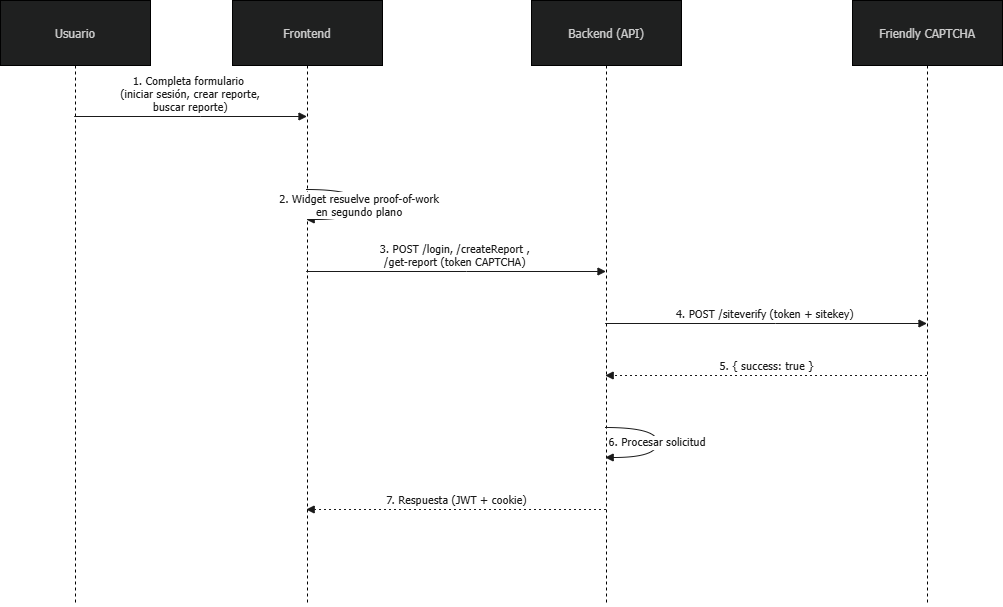
\includegraphics[width=0.85\textwidth]{Graphics/Cap4/captcha_completo.png}
    \caption{Flujo de verificación de Friendly CAPTCHA en endpoints públicos.}
    \label{fig:captcha_flow}
\end{figure}


\subsubsection{Limitación de velocidad}

La limitación de velocidad (en inglés, \textit{rate limiting}) restringe el número de solicitudes que un cliente puede realizar a la API en un período de tiempo determinado. Su propósito es proteger el sistema contra ataques de fuerza bruta, enumeración de recursos y denegación de servicio \cite{microsoft_rate_limiting}. Además, evita que picos de tráfico legítimo o bucles accidentales en el frontend consuman todos los recursos del servidor y degraden la experiencia del resto de usuarios.

Los endpoints públicos del sistema ya cuentan con CAPTCHA como primera barrera, según se describió anteriormente.
El rate limiting actúa como segunda barrera: si un atacante resuelve el CAPTCHA para cada intento, el límite de solicitudes por minuto hace inviable cualquier ataque masivo. Para los endpoints protegidos con JWT, el rate limiting constituye la defensa principal contra el abuso por parte de usuarios autenticados o tokens comprometidos.

\paragraph{Limitación por IP y por sesión}

El sistema aplica un limitador global que contabiliza todas las solicitudes de un mismo cliente, independientemente del endpoint al que se dirijan. Para clientes anónimos —como un reportante que envía un formulario público—, el límite se aplica por dirección IP: 100 solicitudes por minuto. Para usuarios autenticados, el límite se aplica por identificador de sesión extraído del JWT: 200 solicitudes por minuto. Esta diferenciación evita que usuarios legítimos que comparten red —como el personal de un mismo centro de salud— resulten bloqueados por el comportamiento de un tercero, y otorga mayor margen a quienes ya superaron la barrera de autenticación. Una solicitud solo se procesa si el limitador global lo permite.

\paragraph{Políticas complementarias por tipo de operación}

Sobre esta base, el sistema añade políticas específicas que restringen aún más ciertos endpoints según la criticidad de la operación. 
Cada política define un límite de solicitudes, una ventana de tiempo y un comportamiento de encolamiento. 
La ventana fija restablece el contador al cumplirse el intervalo; la ventana deslizante distribuye el límite en segmentos para suavizar los picos de tráfico legítimo. 
El encolamiento permite retener las solicitudes excedentes durante un breve período antes de rechazarlas, lo que evita que un pico puntual de actividad legítima genere errores inmediatos al cliente \cite{microsoft_rate_limiting}.

\begin{itemize}
    \item \texttt{Auth}: 3 solicitudes por minuto para endpoints de autenticación, sin encolamiento. Un usuario legítimo inicia sesión pocas veces al día; tres intentos por minuto bastan para la operación normal y hacen inviable un ataque de fuerza bruta incluso si el atacante resuelve el CAPTCHA en cada intento.
    \item \texttt{Command}: 5 solicitudes por minuto para operaciones de escritura estándar, como la creación de reportes ESAVI, con cola de hasta 5 solicitudes. Equivale a un reporte cada 12 segundos, ritmo suficiente para un centro de salud con múltiples reportantes simultáneos.
    \item \texttt{ReportDaily}: 30 solicitudes por día para la creación de reportes desde una misma IP, mediante ventana deslizante de 24 horas dividida en 24 segmentos. Cubre la actividad diaria de un centro de salud activo y acota el daño máximo de un ataque automatizado a 30 reportes falsos, los cuales pueden identificarse y eliminarse manualmente.
    \item \texttt{CommandDaily}: 20 solicitudes por día para operaciones administrativas como la asignación de reportes o la finalización de revisiones médicas. Refleja el ritmo real de trabajo de un jefe de vacunación municipal o médico evaluador.
    \item \texttt{Query}: 60 solicitudes por minuto para operaciones de lectura, con ventana deslizante dividida en 3 segmentos y cola de hasta 10 solicitudes. Las consultas no modifican el estado del sistema; una consulta por segundo permite una navegación fluida mientras dificulta la extracción masiva de datos.
\end{itemize}

El siguiente fragmento muestra la configuración de dos de estas políticas dentro de la clase \texttt{RateLimitingMiddleware}:

\begin{lstlisting}[language={[Sharp]C}, caption={Configuración de políticas de rate limiting}, label={lst:ratelimiting}]
// Autenticación: muy restrictivo
options.AddFixedWindowLimiter("Auth", config =>
{
    config.PermitLimit = 3;
    config.Window = TimeSpan.FromMinutes(1);
    config.QueueProcessingOrder = QueueProcessingOrder.OldestFirst;
    config.QueueLimit = 0;
});

// Comandos estándar: restrictivo
options.AddFixedWindowLimiter("Command", config =>
{
    config.PermitLimit = 5;
    config.Window = TimeSpan.FromMinutes(1);
    config.QueueProcessingOrder = QueueProcessingOrder.OldestFirst;
    config.QueueLimit = 5;
});
\end{lstlisting}




\paragraph{Aplicación a endpoints}
El atributo \texttt{[EnableRate\-Limiting]} aplica las políticas sobre controladores completos o endpoints específicos. Un mismo endpoint puede combinar múltiples políticas cuando requiere protección en distintas ventanas de tiempo. Por ejemplo, el controlador de autenticación declara únicamente \texttt{Auth} a nivel de clase:

\begin{lstlisting}[language={[Sharp]C}, caption={Aplicación del rate limiting a controladores y endpoints}, label={lst:ratelimitingapplication}]
[ApiController]
[Route("api/[controller]")]
[EnableRateLimiting("Auth")]
public class AuthenticationController : ControllerBase { }
\end{lstlisting}

El endpoint de creación de reportes, en cambio, combina dos políticas: \texttt{Command} limita la tasa por minuto y \texttt{ReportDaily} impone un límite diario por IP. Ambas se evalúan en conjunto con el limitador global: la solicitud solo se procesa si las tres capas lo permiten.

\begin{lstlisting}[language={[Sharp]C}, caption={Combinación de políticas en un mismo endpoint}, label={lst:ratelimitingcombination}]
[HttpPost]
[EnableRateLimiting("Command")]
[EnableRateLimiting("ReportDaily")]
public async Task<IActionResult> Create(CreateReportDto dto) { }
\end{lstlisting}


\paragraph{Alcance de las defensas implementadas}

Aun con estas barreras, un atacante necesitaría resolver múltiples desafíos de proof-of-work y mantenerse por debajo de los umbrales de rate limiting simultáneamente. 
El costo computacional de esta estrategia la vuelve inviable para ataques masivos con los recursos actuales.



















\section{Implementación de la interfaz de usuario}
\label{section:frontend}

El frontend del sistema se construye como una Single Page Application (SPA) en React con TypeScript. La aplicación consume la API REST del backend y ofrece una interfaz accesible tanto para la población que reporta eventos adversos como para el personal del Instituto Finlay que gestiona las revisiones.

\subsection{Arquitectura y enrutamiento}

La aplicación utiliza enrutamiento interno sin depender de librerías externas como React Router. Un componente principal mantiene el estado de la página actual y sincroniza la ruta del navegador con el componente correspondiente mediante un mapa de rutas. Esta decisión reduce el tamaño del bundle final y permite animaciones de transición entre páginas. El acceso a las páginas restringidas se protege mediante un contexto de autenticación que redirige al usuario a la página de inicio de sesión si no hay una sesión activa. Los contextos globales de autenticación y reportes envuelven toda la aplicación y comparten el estado sin necesidad de pasarlo manualmente entre componentes.

\subsection{Gestión del estado y comunicación con la API}

El estado global de autenticación reside en un contexto de React que expone los datos del usuario, el estado de la sesión y las funciones de inicio y cierre de sesión. Al cargar la aplicación, este contexto intenta restaurar la sesión mediante el endpoint de refresco de token, lo que evita que el usuario deba iniciar sesión nuevamente si su token de acceso expiró.

La comunicación con el backend se centraliza en una instancia de Axios configurada con interceptores para la gestión automática de tokens. El interceptor de solicitud inyecta el encabezado de autorización con el token de acceso; el interceptor de respuesta detecta los códigos 401, intenta renovar el token y reenvía la solicitud original. El refresco excluye los endpoints de autenticación para evitar bucles y preserva los encabezados originales en el reintento. Si la renovación falla, la sesión se cierra automáticamente y el usuario regresa a la página de inicio de sesión.

\subsection{Almacenamiento del JWT en memoria}

El token de acceso se mantiene exclusivamente en memoria, sin persistencia en almacenamiento local o de sesión. Esta decisión reduce el riesgo de robo por lecturas desde almacenamiento persistente, aunque no protege contra scripts inyectados que se ejecuten en la página. Por ello, el patrón de seguridad completo combina el token de acceso en memoria con un refresh token almacenado en una cookie HttpOnly, Secure y con SameSite estricta, que el frontend no manipula y por tanto no es vulnerable a ataques de cross-site scripting.

Esta estrategia conlleva un riesgo: el token de acceso se pierde al recargar la página. Para mitigarlo, el contexto de autenticación invoca el endpoint de refresco al cargar la aplicación. Si el refresco tiene éxito, el nuevo token se almacena en memoria y la sesión se restaura sin interrupción para el usuario.

\subsection{Validación en tiempo real}

Los formularios del sistema aplican validación en tiempo real mediante las librerías \texttt{react-hook-form} y \texttt{zod}. La primera reduce el número de renderizaciones al no almacenar el estado de cada campo individualmente, lo que mejora el rendimiento en formularios extensos como el de registro de reportes. La segunda define esquemas declarativos que especifican el formato esperado de cada campo —correo electrónico válido, longitud mínima de contraseña, coincidencia entre campos— y los mensajes de error correspondientes. La integración de ambas permite que el usuario reciba retroalimentación inmediata mientras escribe, sin esperar a enviar el formulario, lo que reduce la cantidad de solicitudes fallidas al backend y mejora la experiencia de uso.

\subsection{Construcción de interfaces de usuario y diseño responsivo}

La interfaz se compone de componentes reutilizables construidos con Tailwind CSS y Radix UI. Tailwind CSS proporciona utilidades de diseño que permiten crear interfaces responsivas sin escribir hojas de estilo personalizadas: las cuadrículas reorganizan sus columnas según el ancho de la pantalla, la navegación alterna entre un menú de escritorio y un menú lateral en dispositivos móviles, y los formularios mantienen un aspecto adecuado en cualquier tamaño de pantalla. Radix UI aporta componentes accesibles —diálogos, selectores, pestañas— que garantizan la compatibilidad con lectores de pantalla y navegación por teclado, en cumplimiento de los requisitos de accesibilidad.

Los gráficos del panel de control utilizan \texttt{recharts}, una librería de visualización de datos para React. Cada gráfico se envuelve en un contenedor responsivo que adapta su tamaño al ancho disponible, y los datos se preprocesan en el backend para reducir el volumen de información transferida al cliente. Los componentes visuales emplean memoización para evitar renderizaciones innecesarias y mantener un rendimiento fluido durante la navegación.

\subsection{Manejo de autenticación en el cliente}

Al iniciar sesión, el cliente decodifica el JWT para extraer el rol del usuario y mostrar únicamente las rutas y opciones correspondientes a ese perfil. 
Esta diferenciación garantiza que cada perfil acceda exclusivamente a las funcionalidades que le corresponden, en cumplimiento de los requisitos de autorización definidos en el Capítulo \ref{chapter:proposal}.



% \section{Implementación del frontend}
% \label{section:frontend}

% El frontend del sistema se construye como una Single Page Application (SPA) en React con TypeScript. La aplicación consume la API REST del backend y ofrece una interfaz accesible tanto para la población que reporta eventos adversos como para el personal del Instituto Finlay que gestiona las revisiones.

% \subsection{Arquitectura y enrutamiento}

% La aplicación utiliza enrutamiento interno controlado por el componente principal \texttt{App.tsx}, que mantiene el estado de la página actual y sincroniza la ruta del navegador con el componente correspondiente mediante un mapa de rutas. Esta decisión evita la dependencia de librerías externas de enrutamiento, reduce el tamaño del bundle final y permite animaciones de transición entre páginas. El acceso a las páginas restringidas se protege mediante el contexto de autenticación (\texttt{AuthContext.tsx}), que redirige al usuario a la página de inicio de sesión si no hay una sesión activa. Los contextos \texttt{AuthProvider} y \texttt{ReportProvider} envuelven toda la aplicación y comparten el estado global sin necesidad de pasarlo manualmente entre componentes.

% \subsection{Gestión del estado y comunicación con la API}

% El estado global de autenticación reside en \texttt{AuthContext.tsx}, que expone los datos del usuario, el estado de la sesión y las funciones de inicio y cierre de sesión. Al cargar la aplicación, el contexto intenta restaurar la sesión mediante el endpoint de refresco de token, lo que evita que el usuario deba iniciar sesión nuevamente si su token de acceso expiró.

% La comunicación con el backend se centraliza en una instancia de Axios (\texttt{api.ts}) configurada con interceptores para la gestión automática de tokens. El interceptor de solicitud inyecta el encabezado \texttt{Authorization} con el token de acceso; el interceptor de respuesta detecta los códigos 401, intenta renovar el token mediante el servicio de autenticación (\texttt{auth.service.ts}) y reenvía la solicitud original. El refresco excluye explícitamente los endpoints de autenticación para evitar bucles, y preserva los encabezados originales en el reintento:

% \begin{lstlisting}[language={TypeScript}, caption={Interceptores de Axios para manejo de tokens (api.ts)}, label={lst:axios}]
% api.interceptors.request.use((config) => {
%     const token = tokenManager.getAccessToken();
%     if (token) config.headers.Authorization = `Bearer ${token}`;
%     return config;
% });

% api.interceptors.response.use(
%     (response) => response,
%     async (error) => {
%         const originalRequest = error.config;
%         if (error.response?.status === 401 
%             && !originalRequest._retry
%             && !originalRequest.url?.includes('/Authentication/')) {
%             originalRequest._retry = true;
%             try {
%                 const { accessToken } = await authService.refreshToken();
%                 tokenManager.setAccessToken(accessToken);
%                 originalRequest.headers.Authorization = `Bearer ${accessToken}`;
%                 return api(originalRequest);
%             } catch (refreshError) {
%                 tokenManager.clearAccessToken();
%                 window.location.href = '/login';
%                 return Promise.reject(refreshError);
%             }
%         }
%         return Promise.reject(error);
%     }
% );
% \end{lstlisting}

% \subsection{Almacenamiento del JWT en memoria}

% El token de acceso se mantiene en memoria mediante el módulo \texttt{token-manager.ts} para evitar su persistencia en \texttt{localStorage} o \texttt{sessionStorage}. Esta decisión reduce el riesgo de robo por lecturas desde almacenamiento persistente, aunque no protege contra scripts inyectados que se ejecuten en la página. Por ello, el patrón de seguridad completo combina el token de acceso en memoria con un refresh token almacenado en una cookie HttpOnly, Secure y con SameSite estricta, que el frontend no manipula y por tanto no es vulnerable a XSS.

% Esta estrategia conlleva un riesgo: el token de acceso se pierde al recargar la página. Para mitigarlo, el contexto de autenticación invoca el endpoint de refresco al cargar la aplicación. Si el refresco tiene éxito, el nuevo token de acceso se almacena en memoria y la sesión se restaura sin que el usuario perciba interrupción alguna. El backend debe reforzar esta protección aplicando tasas límite al endpoint de refresco, rotando los refresh tokens y revocándolos ante uso indebido.

% \subsection{Validación en tiempo real}

% Los formularios del sistema —presentes en páginas como \texttt{login-page.tsx} y \texttt{activate-account-page.tsx}— aplican validación en tiempo real mediante las librerías \texttt{react-hook-form} y \texttt{zod}. \texttt{react-hook-form} reduce el número de renderizaciones al no almacenar el estado de cada campo individualmente, lo que mejora el rendimiento en formularios extensos como el de registro de reportes. \texttt{zod} define esquemas declarativos que especifican el formato esperado de cada campo y los mensajes de error correspondientes. La integración de ambas librerías mediante \texttt{@hookform/resolvers} permite que el usuario reciba retroalimentación inmediata mientras escribe, sin esperar a enviar el formulario:

% \begin{lstlisting}[language={TypeScript}, caption={Validación en tiempo real con react-hook-form y zod}, label={lst:validation}]
% import { useForm } from 'react-hook-form';
% import { z } from 'zod';
% import { zodResolver } from '@hookform/resolvers/zod';

% const schema = z.object({
%     email: z.string().email('Email inválido'),
%     password: z.string().min(8, 'Mínimo 8 caracteres'),
%     confirmPassword: z.string(),
% }).superRefine(({ password, confirmPassword }, ctx) => {
%     if (password !== confirmPassword)
%         ctx.addIssue({
%             code: 'custom',
%             message: 'Las contraseñas no coinciden',
%             path: ['confirmPassword']
%         });
% });

% function AccountForm() {
%     const { register, handleSubmit, formState } = useForm({
%         resolver: zodResolver(schema),
%         mode: 'onChange',
%     });

%     return (
%         <form onSubmit={handleSubmit(onSubmit)}>
%             <input {...register('email')} />
%             {formState.errors.email && <span>{formState.errors.email.message}</span>}
%             <button type="submit" disabled={!formState.isValid}>Enviar</button>
%         </form>
%     );
% }
% \end{lstlisting}

% \subsection{Construcción de interfaces de usuario y diseño responsivo}

% La interfaz se compone de componentes reutilizables construidos con Tailwind CSS y Radix UI, una librería de componentes accesibles que garantiza la compatibilidad con lectores de pantalla y navegación por teclado. Cada página —inicio de sesión, activación de cuenta, panel de reportes, formulario de registro— se implementa como un componente independiente que consume los contextos globales y los servicios de API.

% La responsividad se logra mediante las utilidades de Tailwind CSS. Las cuadrículas reorganizan sus columnas según el ancho de la pantalla, la navegación alterna entre un menú de escritorio y un menú lateral en dispositivos móviles, y los gráficos del panel de control utilizan \texttt{ResponsiveContainer} de \texttt{recharts} para adaptarse automáticamente al tamaño del contenedor. Para garantizar un rendimiento fluido, los datos de los gráficos se preprocesan en el backend y los componentes visuales emplean \texttt{useMemo} para evitar renderizaciones innecesarias. El siguiente fragmento muestra un gráfico de líneas responsivo:

% \begin{lstlisting}[language={TypeScript}, caption={Gráfico responsivo con recharts}, label={lst:recharts}]
% <ResponsiveContainer width="100%" height={300}>
%     <LineChart data={eventsByMonth}>
%         <CartesianGrid strokeDasharray="3 3" />
%         <XAxis dataKey="month" />
%         <YAxis />
%         <Tooltip />
%         <Line type="monotone" dataKey="total" stroke="#0A4B8F" />
%     </LineChart>
% </ResponsiveContainer>
% \end{lstlisting}

% \subsection{Manejo de autenticación en el cliente}

% Al iniciar sesión, el cliente decodifica el JWT para extraer el rol del usuario y mostrar únicamente las rutas y opciones correspondientes a ese rol. El componente de navegación (\texttt{navigation.tsx}) utiliza \texttt{useAuth()} para renderizar menús diferentes según el perfil: un jefe de vacunación ve opciones de asignación y estadísticas; un revisor médico ve únicamente los reportes asignados; un ciudadano solo accede al formulario de reporte público y a la consulta por número de notificación.






% \section{Implementación de funcionalidades principales}
% \label{section:functionalities}

% \subsection{Registro de reportes de ESAVI}

% \subsection{Gestión de revisiones médicas}

% \subsection{Asignación de responsables}

% \subsection{Gestión de causalidad}

% \subsection{Sistema de notificaciones}

% \subsection{Visualización y consulta de reportes}

\section{Despliegue de la solución}
\label{section:deployment}

El sistema se despliega en dos entornos diferenciados. Para desarrollo local, un archivo \texttt{docker-compose.yml} levanta los servicios de RabbitMQ y la API, mientras que la base de datos MySQL se ejecuta en el servidor local. 
Para demostración y pruebas, la API se despliega en Railway, una plataforma como servicio que automatiza la construcción y publicación desde el repositorio de GitHub. 

La configuración se centraliza en un \texttt{Dockerfile} multietapa\footnote{Multietapa: técnica que divide la construcción en fases con imágenes base distintas, reduciendo el tamaño final.} que compila la aplicación en una imagen de SDK\footnote{SDK: imagen con compilador y herramientas de desarrollo.} y la publica en una imagen de runtime\footnote{Runtime: imagen solo con las bibliotecas para ejecutar la aplicación.}, y en variables de entorno que inyectan las credenciales de base de datos, las claves de JWT y las API keys de los servicios externos sin exponerlas en el código fuente.

La migración a servidores físicos del Instituto Finlay, prevista para la etapa de producción, mantendrá la misma configuración de contenedores y variables de entorno, lo que garantiza que el entorno de producción sea idéntico al de desarrollo.



\section{Conclusiones del capítulo}
\label{section:chapter_conclusions}

En este capítulo se presentaron los principales detalles relacionados con la implementación de la plataforma desarrollada, describiendo las tecnologías empleadas, la organización arquitectónica de la solución y los mecanismos utilizados en el backend y el frontend. Además, se abordaron aspectos asociados a la seguridad, la integración entre componentes y el despliegue del sistema, evidenciando la materialización práctica de la propuesta presentada en el capítulo anterior.
